\documentclass[a2paper]{article}
\usepackage[fontsize=13.9pt]{fontsize}
\usepackage[margin=1cm,landscape]{geometry}
% \documentclass[a4paper]{article}
\usepackage{fontspec}
\usepackage[]{flowfram}
\usepackage{graphicx}
\usepackage{tabularx}
\usepackage{hyperref}
\usepackage{booktabs}
\ffvadjustfalse
\setlength{\columnsep}{1cm}
\Ncolumn{3}

\author{Xiyan Shao}
\title{Towards Unsupervised Few-Shot Text Style Transfer: \\ A Method with Pretrained LM and Style Extractor}
\begin{document}
\maketitle
\section{Introduction}
Responding to different contexts and audiences, people speak and write in different styles. A naturally occurring linguistic variation, style is defined by a large set of attributes of texts, which includes but is not limited to formality, politeness, diction, and emotion.

Text style transfer (TST) is a task in NLP which aims to change certain attributes in the style of a text while preserving its meaning. A task with a long history, it has significant applications for downstream tasks like machine translation, in which it can help reduce the difficulty of interpreting stylistic texts; text simplification, in which it translates complicated text for a wider audience; and formality transfer, in which it helps modifying the formality of text for different social contexts. Table \ref{tab:original_and_stylized_text} shows some transfer examples.

However, unlike the well-known success in image style transfer, the progress of text style transfer has been greatly limited by the discrete nature of text data and, more crucially, the lack of parallel training data. As identified by many researchers, a key problem in the TST task is how to develop unsupervised models that can make use of the abundant unlabeled training data which enabled training huge language models like BERT, T5, GPT, and so on.

% insert table of two columns, one for original text, one for stylized text
\begin{table}[h!]
\centering
\label{tab:original_and_stylized_text}
\begin{tabularx}{\linewidth}{XX}
Original text & Stylized text \\ \midrule 
(Rude) What the hell is wrong with your attitude? & (Polite) Perhaps the question is more about your attitude.\\
(Positive) Apple's new chip worths it's price. & (Negative) Apple's new chip is to expensive to afford.\\
\end{tabularx}
\caption{Example of text style transfer tasks}
\label{tab:original_and_stylized_text}
\end{table}

\section{Methodology}

In this project, I aimed to leverage large pre-trained language models and approach the TST task with transformer-based models. After experimenting with a naive seq2seq model based on T5 with a language model head and a Generator-Discriminator network that enables adversarial training, I ended up developing and training a T5 based conditional generation model with a language model head and a style extractor encoder.

\subsection{Model Architecture}

The idea of the final model is based on the TextSETTR paper. Since the authors did not release their source code, from scratch, I implemented a T5ForConditionalGenerationWithExtractor model by extending the vanilla T5 model from the huggingface/transformers repository. Following the TextSETTR model architecture, I made multiple changes (e.g., noise generation function, extractor specifications, and hyperparameters) to the author's idea, and achieved a working and probably the first third-party implementation of T5 based text style extraction model. The model definition is on the right.
\begin{figure}[h!]
    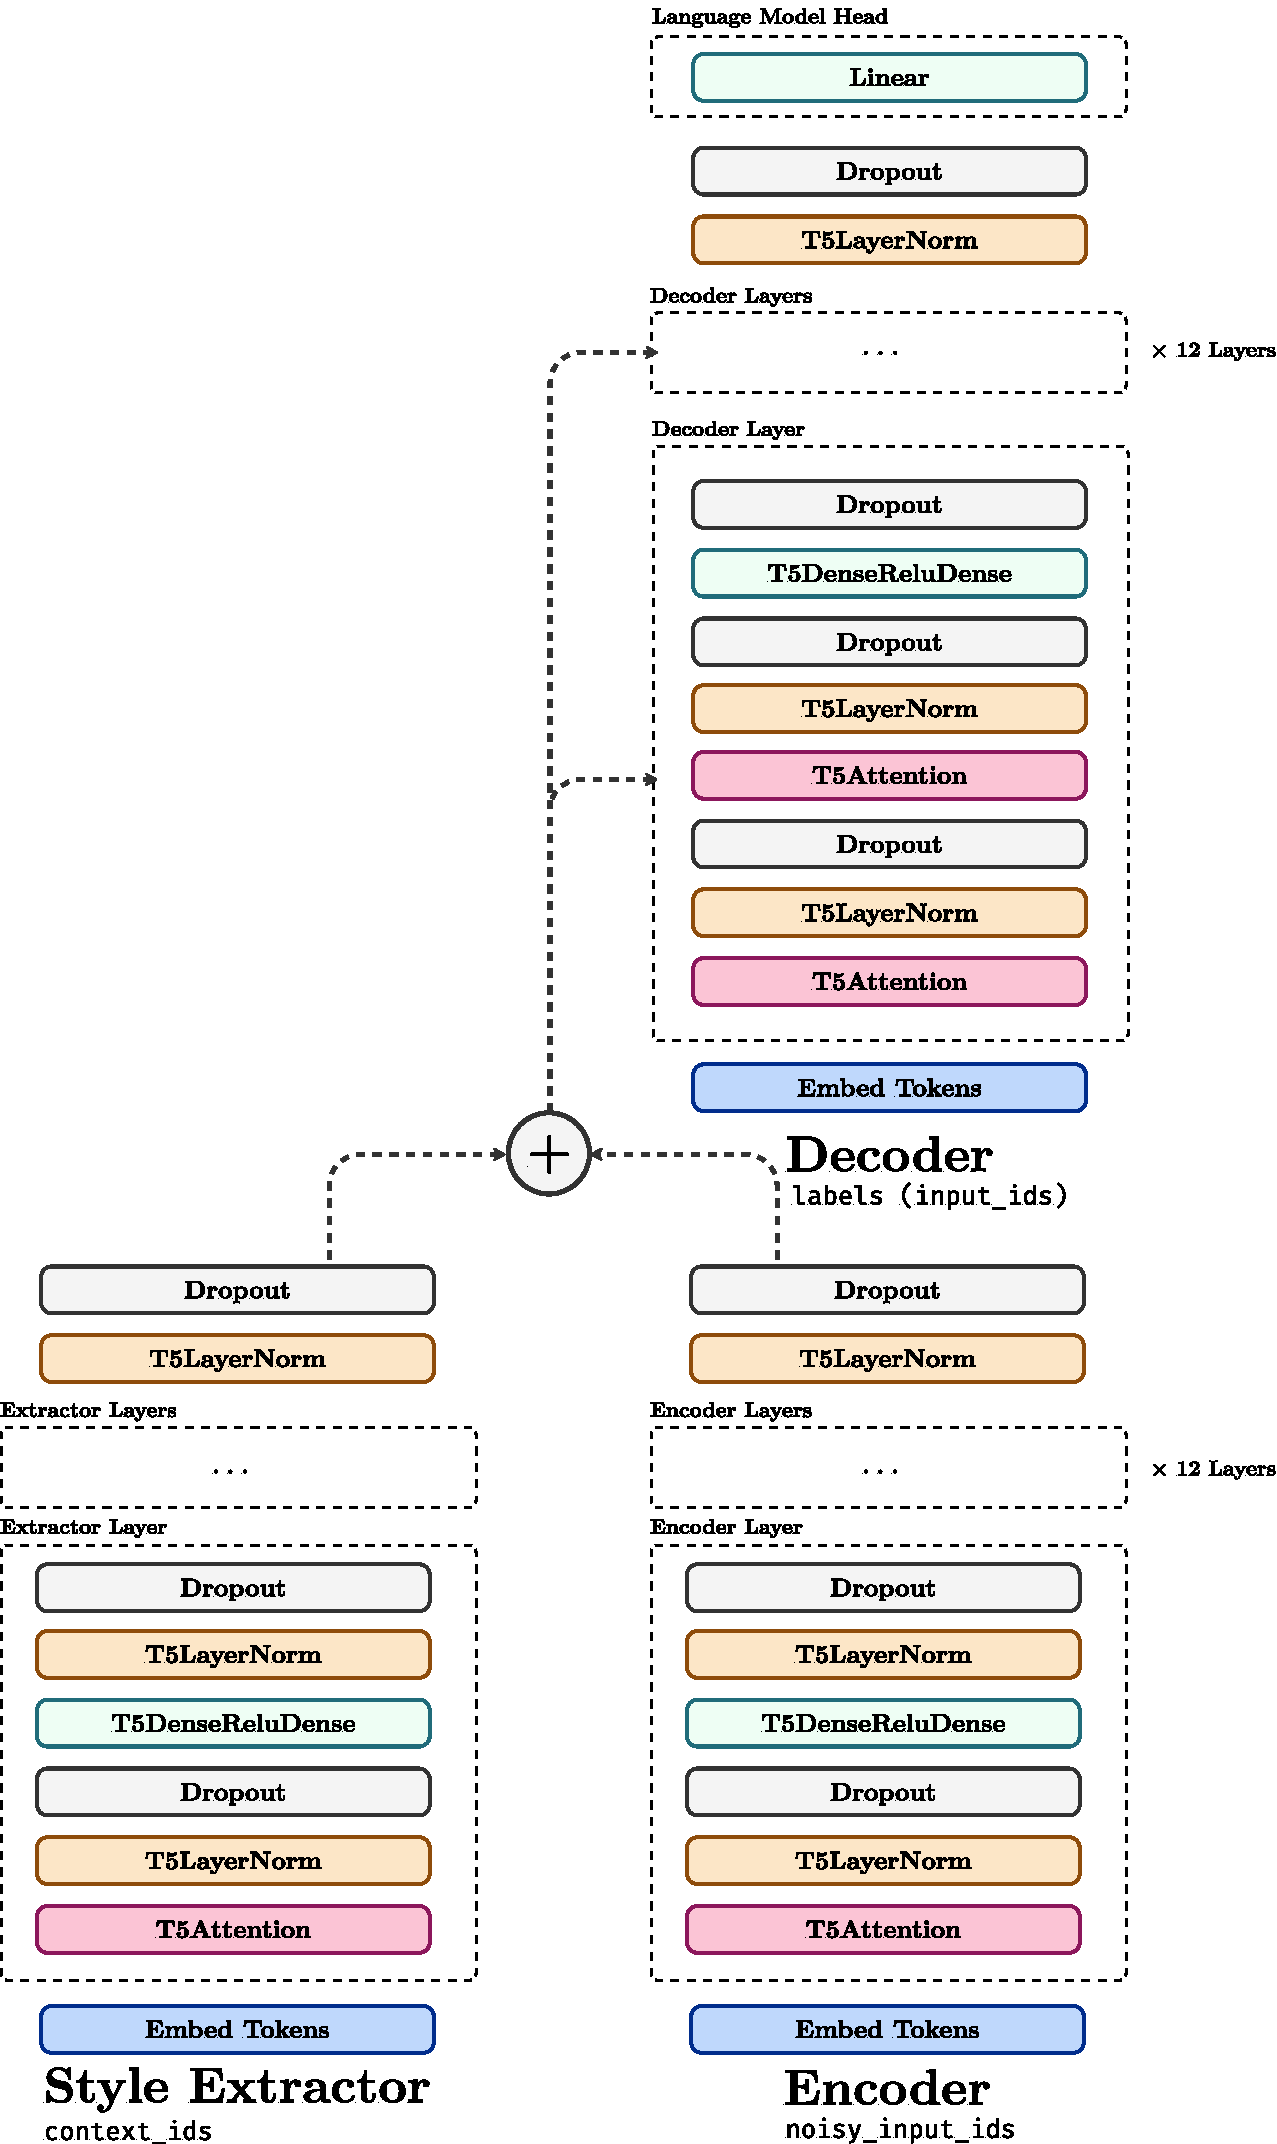
\includegraphics[width=\linewidth]{model_df.pdf}
    \caption{T5ForConditionalGenerationWithExtractor}
    \label{fig:T5ForConditionalGenerationWithExtractor}
\end{figure}

\subsection{Data Preparation}
To train the model, I used the \href{https://nijianmo.github.io/amazon/index.html}{Amazon Review Data (2018)} dataset. Since the whole dataset is too large, I randomly sampled one million lines from the 5-core sub dataset. The dataset is preprocessed by only taking reviews with $\ge$ 2 sentences, where each sentence has 30 or more characters. I implemented a PyTorch Dataset class to load the dataset and preprocess the data, and for every pair of sentences in the dataset, the first sentence is used as the context and the second sentence the as the input. Finally, I tokenized the sentences using the original T5 tokenizer, split up the training, validation, and testing datasets, and created a Pytorch Lightning DataModule for batching and training.

\subsection{Training}
The training of T5ForConditionalGenerationWithExtractor is unsupervised and facilitated by a denoising task. I implemented helper functions to add noise to the input sentence (one for adding noisy tokens (40\%) and another one for randomly dropping tokens (20\%)). Like the original paper method, I also employed the Noisy Back Translation technique (same amount as the mechanical noises) to improve the transfer accuracy. The diagram above shows the training process data flow of the training process. The preceding sentence tokens are used for the context, and the following sentence tokens with Drop/Add + NBT noise are used as the input IDs. With the training goals being to reconstruct the noisy text based on the context style, the ground true sentences are directly fed into the decoder for a cross-entropy loss after the linear language model head. For hyperparameters, I used the AdamW optimizer with a learning rate of 1e-3 and Pytorch Lightning's automatic scheduler. The batch size is set to 32, the maximum number of tokens is also set to 32. Because there's only one available GPU on Google Colab and there are over 332 million trainable parameters, I trained the model for merely 2 epochs.

\begin{figure}[h!]
    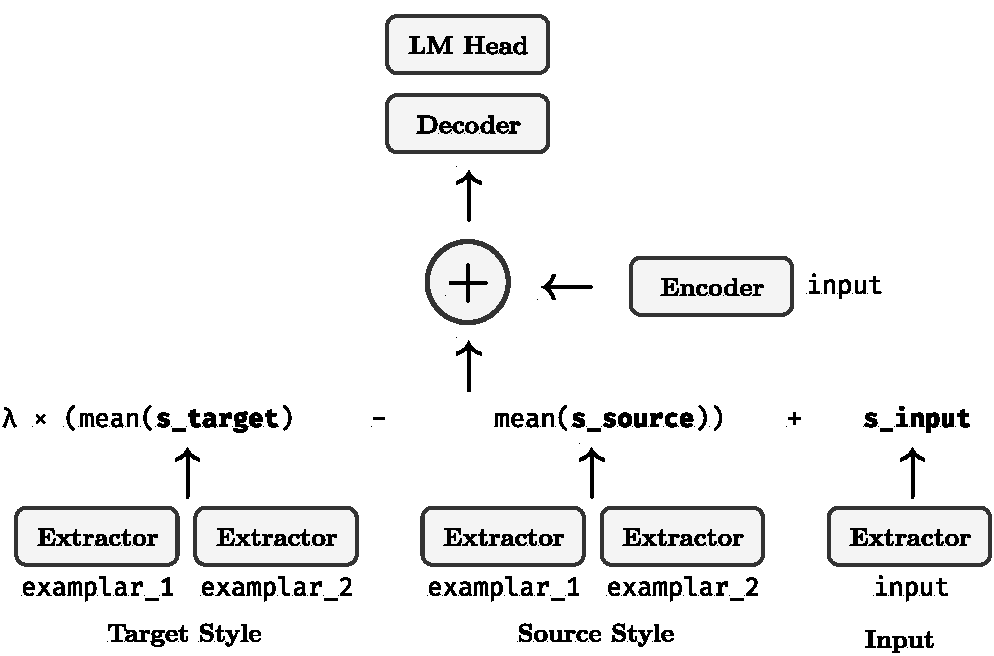
\includegraphics[width=\linewidth]{eval.pdf}
\end{figure}

In evaluation mode, the strategy illustrated in the figure above is used to transfer text styles on a few-shot basis. First, we choose a style target style and also a source style similar to the input style. We feed the extractor with exemplars for both styles and get the corresponding style embeddings, and by subtracting the target style embedding from the source style embedding, we get a style vector pointing towards the target style. In this way, by adding the style direction to the extracted input style, we can get the transferred style. The style vector is then summed with the input encoder's final hidden states to get the final embedding, which is to be decoded. After a greedy search for the language model output, we get the predicted output sentence.

\section{Results}

\begin{table}[h!]
    \centering
    \label{tab:result}
    \begin{tabularx}{\linewidth}{XX}
    Original text & Stylized text \\  \midrule
    (Formal) I hereby commit to never purchase anything from this institution in the future. & (Informal) I'm hereby going to never buy from this seller again.\\
    (Formal) I couldn’t figure out what the author was trying to say. & (Formal) I couldn't figure out what exactly the author was trying to say. \newline (Informal) I couldnt figure out what the author was trying to say.\\
    (Prompt) My favorite movie is & (Emotional) My favorate movie is awesome. My Favorate Movie is amazing! \newline (Reserved) My favorate movie is the movie which is great.\\
    \end{tabularx}
    \caption{Example of text style transfer tasks}
\end{table}

The examples above show the transfer results of the model. The first two lines show a task of formal $\leftrightarrow$ informal transfer, and all the outputs are generated by conditioning on only 3 exemplars for each style for example. We can observe that the first result is pretty remarkable, and the second result shows the flexibility of transfer directions (target style not necessarily $\ne$ input style) -- for formal $\rightarrow$ informal, notice that it spells \textit{couldn’t} as \textit{couldnt}, a sign of informal language.

The last example shows that this model of capable of conditional generation tasks rather than mere seq2seq. Provided with prompt and conditioned on 3 examples in each style category, the generated texts differ by their level of emotion.

Nonetheless, from the example above, one can also see that the generation accuracy is questionable (e.g., last sentence). This is probably limited by the amount of training data (I only used less than 1/100 of the original dataset) and the insufficient training steps. Also, I used the t5-base model instead of t5-large because of the limited CUDA memory -- this could potentially reduce the power of the language model.
\end{document}